\subsubsection{Funktionsweise}
Bei der Bilderzeugung, ausgehend von Szenen, welche viel Geometrie beinhalten bzw. bei Szenen 
die generelle BRDF's verwenden eignet sich das \ref{ch:Content1:sec:PathTracer}path tracing \cite{kajiya1986rendering}.
Das \ref{ch:Content1:sec:PathTracer}path tracing ist in Hinsicht der Beleuchtung komplett. Deshalb lässt sich damit
\textit{Global Illumination} erreichen. Das hier verwendete \ref{ch:Content1:sec:PathTracer}path tracing in 
\cite[eragae]{Benty18} verwendet eine klassische Umsetzung.\par

\begin{figure}[H]
    \centering
    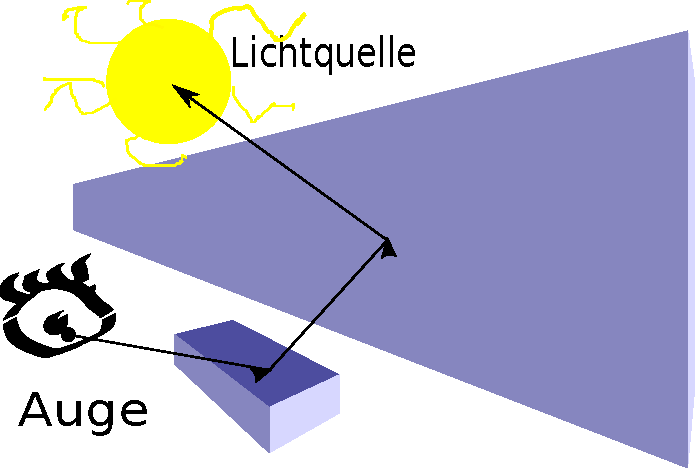
\includegraphics[width=0.7\linewidth]{content/PathTracer/Bilder/Grundkonzept_path_tracing.pdf}
    \label{pic::PathTracingGrundkonzept}
    \caption{Grundkonzept path tracer}
\end{figure}


Wie in \cite{marschner2009fundamentals} beschrieben wird ausgehend von der vollständigen Transportgleichung
\begin{equation}
    L_s(k_0) = L_e(k_0) + \int_{all(k_i)}^{} \rho(k_i, k_0)*L_f(k_i)*cos(\theta_i)d\theta_i
\end{equation}
    
\begin{equation}
        L(x,{x}^{'}) = g(x,{x}^{'}) * (L_{e}(x,{x}^{'}) + 
                        \int_{S}^{} b(x,{x}^{'},{x}^{''})
                        L({x}^{'},{x}^{''}d{x}^{''})) 
\end{equation}
Sie beschreibt den Energietransport \textit{L(x,${x}^{'})$} von einem Punkt ${x}^{'}$
zu einem Punkt x. Dabei ist ein maßgebender Faktor, die relative Lage der beiden Punkte
zueinander im Raum $g(x,{x}^{'})$. Ein weiterer Faktor ist die Abstrahlung 
$L_{e}(x,{x}^{'})$ von ${x}^{'}$ nach x. Beinflusst wird der Energiefluss auch durch
die bidirektionale Verteilungsfunktion $b(x,{x}^{'},{x}^{''})$, welche Aufschluss über
das einfallende Licht von einem Punkt ${x}^{''}$ über ${x}^{'}$ zu x.

\subsubsection{Monte-Carlo-Integration}
Mit der Monte Carlo Integration approximieren wir die Rendergleichung.\par 
Bei gegebener Funktion \textit{f }:\textit{ S}$\rightarrow \mathbb{R}$ 
\cite{KK02}
\label{pic:MonteCarloIntegration}
\begin{equation}
    \int_{x\in S} g(x) d\mu \simeq \frac{1}{N}*\sum_{i=1}^{N}\frac{g(x_i)}{p(x_i)}
\end{equation}
    


